\documentclass[11pt]{article}
%\usepackage{amsfonts}
\usepackage{amsmath}
\usepackage{fancybox}%,times}
\usepackage{graphicx,psfrag,epsf}
%\usepackage{amsmath}
\usepackage{enumerate}
\usepackage{graphicx,psfrag}
\usepackage{multirow}
\usepackage{epsfig}
%\usepackage{rotating}
\usepackage{subfigure}
\usepackage{theorem}
\usepackage{natbib,psfrag}
\usepackage{tikz}
\usepackage{xcolor}
\usepackage{kotex}
\newcommand{\blind}{0}
\usepackage{graphicx}
\DeclareGraphicsExtensions{.pdf,.png,.jpg}

\addtolength{\oddsidemargin}{-.75in}%
\addtolength{\evensidemargin}{-.75in}%
\addtolength{\textwidth}{1.5in}%
\addtolength{\textheight}{1.3in}%
%\addtolength{\topmargin}{-.6in}%
\addtolength{\topmargin}{-.8in}%

%\theoremstyle{break}
\newtheorem{The}{Theorem}
\newtheorem{Def}{Definition}
\newtheorem{Pro}{Proposition}
\newtheorem{Lem}{Lemma}
\newtheorem{Cor}{Corollary}
\newtheorem{asp}{Assumption}


\renewcommand{\thefootnote}{\arabic{footnote}}
%\renewcommand{\thefootnote}{\alph{footnote}}
%\renewcommand{\thefootnote}{\roman{footnote}}
%\renewcommand{\thefootnote}{\fnsymbol{footnote}}

\begin{document}


%\bibliographystyle{natbib}

\newcommand{\Ito}{$It\hat{o}$'$s~Lemma$}

\newcommand\ind{\stackrel{\rm ind}{\sim}}
\newcommand\iid{\stackrel{\rm iid}{\sim}}
\renewcommand\c{\mathbf{c}}
\newcommand\y{\mathbf{y}}
\newcommand\z{\mathbf{z}}
\renewcommand\P{\mathbf{P}}
\newcommand\W{\mathbf{W}}
\newcommand\X{\mathbf{X}}
\newcommand\Y{\mathbf{Y}}
\newcommand\Z{\mathbf{Z}}
\newcommand\J{{\cal J}}
\newcommand\B{{\cal B}}
\newcommand\K{{\cal K}}
\newcommand\N{{\rm N}}
\newcommand\bs{\boldsymbol}
\newcommand\bth{\bs\theta}
\newcommand\bbe{\bs\beta}
\renewcommand\*{^\star}

\def\spacingset#1{\renewcommand{\baselinestretch}%
{#1}\small\normalsize} \spacingset{1}


%%%%%%%%%%%%%%%%%%%%%%%%%%%%%%%%%%%%%%%%%%%%%%%%%%%%%%%%%%%%%%%%%%%%%%%%%%%%%%

  \bigskip
  \bigskip
  \bigskip
  \begin{center}
    {\LARGE\bf Jan 03, 2019 }
  \end{center}
  \medskip

%\begin{abstract}
%\end{abstract}

%\noindent%
%{\it Key Words:}  AECM algorithm; Astrophysical data analysis;
%ECME algorithm; Incompatible Gibbs sampler; Marginal data
%augmentation; Multiple imputation; Spectral analysis

\spacingset{1.45}







\section{Conjugate Distribution} 

From Bayes theorem
  \begin{align}
    p(\theta | x) = \frac{p(x|\theta)p(\theta)}{\int p(x|\theta')p(\theta')d\theta'}
  \end{align}
All membets of the exponential family have conjugate priors.




\begin{table}[]
\caption{Discrete}
\begin{tabular}{|c|c|c|c|c|}
\hline
Bernoulli                                                                                          & p (probability)                                                                                  & Beta          & $\alpha ,\beta$          & $\alpha +\sum _{i=1}^{n}x_{i},\beta +n-\sum _{i=1}^{n}x_{i}$                        \\ \hline
Binomial                                                                                           & p (probability)                                                                                  & Beta          & $\alpha ,\,\beta $       & $ \alpha +\sum _{i=1}^{n}x_{i},\,\beta +\sum _{i=1}^{n}N_{i}-\sum _{i=1}^{n}x_{i}$  \\ \hline
\begin{tabular}[c]{@{}c@{}}Negative\\ binomial\\ with known \\ failure number, \\ r\end{tabular}   & p (probability)                                                                                  & Beta          & $\alpha ,\beta$          & $\alpha +\sum _{i=1}^{n}x_{i},\,\beta +rn\!$                                        \\ \hline
Poisson                                                                                            & $\lambda$ (rate)                                                                                 & Gamma         & $\alpha ,\,\beta \!$     & $\alpha +\sum _{i=1}^{n}x_{i},\ \beta +n\!$                                         \\ \hline
Multinomial                                                                                        & \begin{tabular}[c]{@{}c@{}}p (probability \\ vector), \\ k(number of \\ categories)\end{tabular} & Dirichlet     & $\alpha$                 & ${\boldsymbol {\alpha }}+\sum _{i=1}^{n}\mathbf {x} _{i}\!$                         \\ \hline
\begin{tabular}[c]{@{}c@{}}Hypergeometric\\ with known total \\ population size, \\ N\end{tabular} & \begin{tabular}[c]{@{}c@{}}M (number of \\ target members)\end{tabular}                          & Beta-binomial & $n=N,\alpha ,\,\beta \!$ & $\alpha +\sum _{i=1}^{n}x_{i},\,\beta +\sum _{i=1}^{n}N_{i}-\sum _{i=1}^{n}x_{i}\!$ \\ \hline
Geometric                                                                                          & $p_{0}$ (probability)                                                                            & Beta          & $\alpha ,\,\beta \!$     & $\alpha +n,\,\beta +\sum _{i=1}^{n}x_{i}-n\!$                                       \\ \hline
\end{tabular}
\end{table}


\begin{figure}[htbp]
\begin{center}
    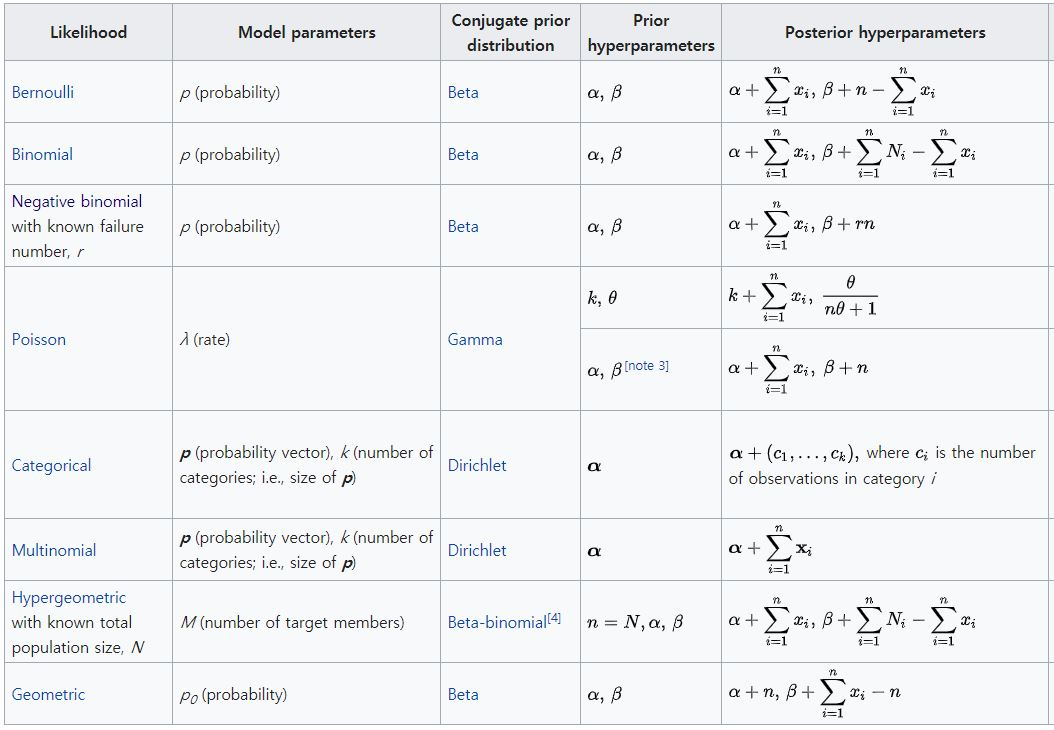
\includegraphics[scale=0.8]{Discrete}
    \caption{Descrete} \label{fig:label}
\end{center}
\end{figure}

\begin{figure}[htbp]
\begin{center}
    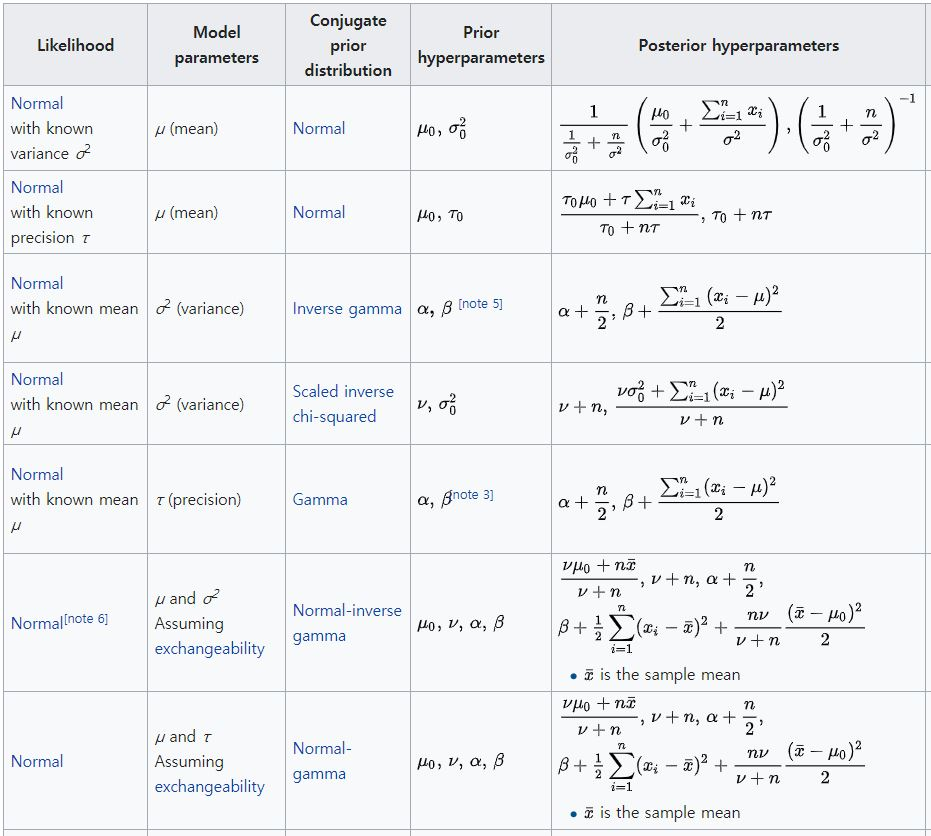
\includegraphics[scale=0.8]{Con1}
    \caption{Continuous 1} \label{fig:label}
\end{center}
\end{figure}

\begin{figure}[htbp]
\begin{center}
    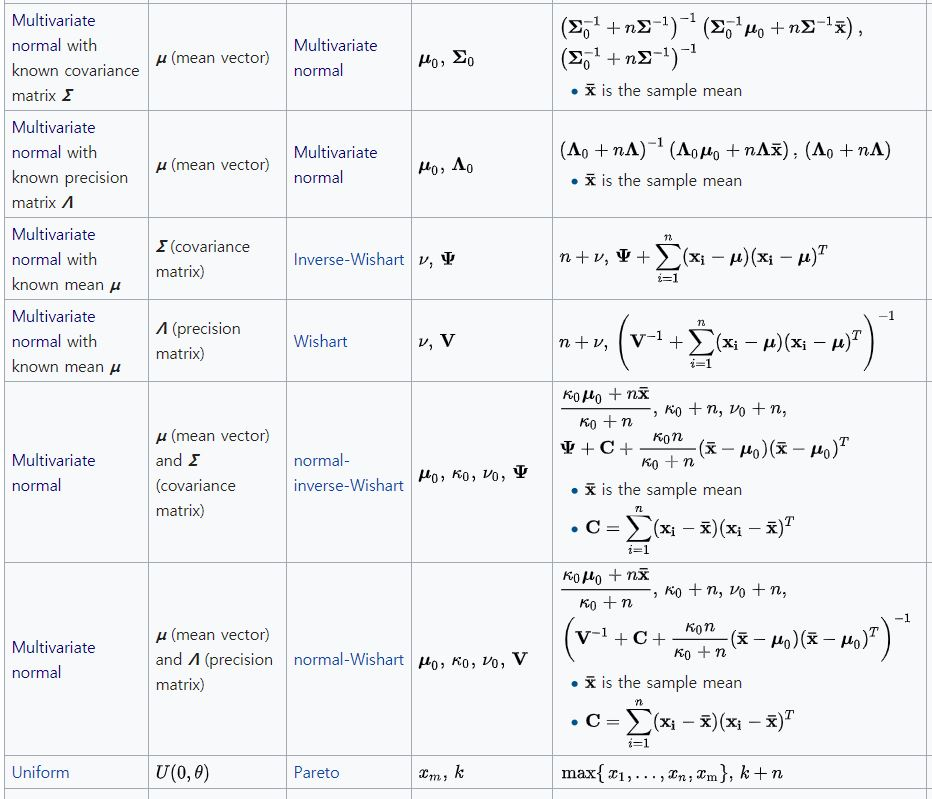
\includegraphics[scale=0.8]{Con2}
    \caption{Continuous 2} \label{fig:label}
\end{center}
\end{figure}

\begin{figure}[htbp]
\begin{center}
    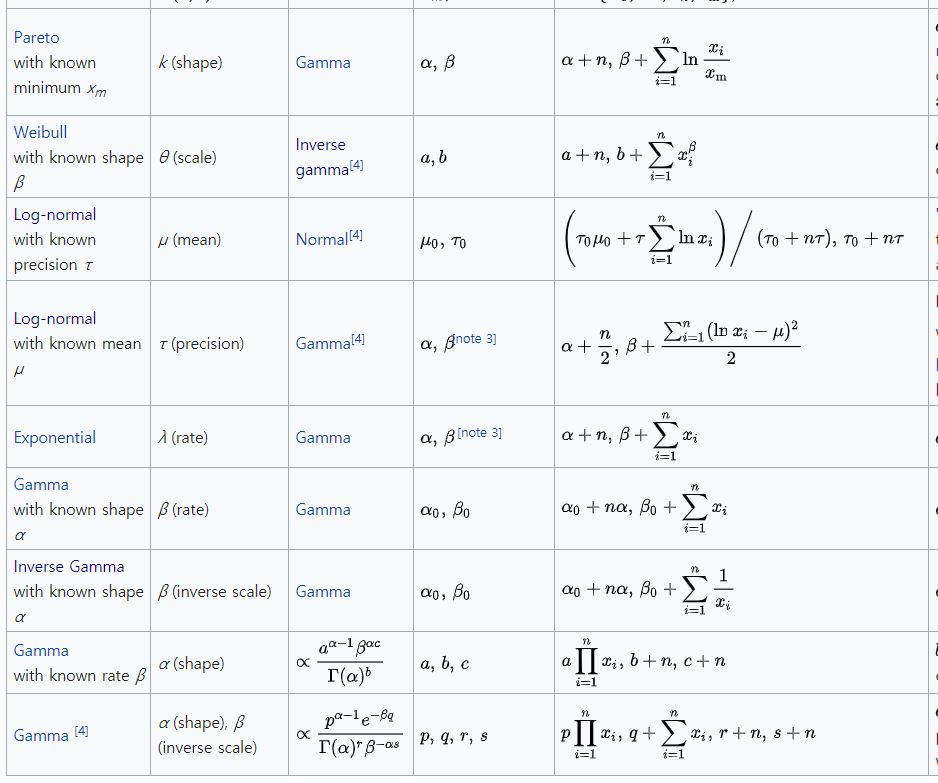
\includegraphics[scale=0.8]{Con3}
    \caption{Continuous 3} \label{fig:label}
\end{center}
\end{figure}

\section{Inverse Distribution} 
$G(y)=\Pr(Y\leq y)=\Pr \left(X\geq {\frac {1}{y}}\right)=1-\Pr \left(X<{\frac {1}{y}}\right)=1-F\left({\frac {1}{y}}\right)$
\end{document}
